\chapter{Аналитический раздел}
В рамках данного раздела представлено описание предметной области задачи по извлечению ключевых слов. Приведена систематизация методов извлечения КС и текстов.
Произведен отбор и сравнение методов удовлетворяющих выставленным ограничениям.
Описана модификация метода Yake

\subsection{Задача автоматического извлечения ключевых слов из текста на естественном языке}

Первые попытки теоретического решения проблемы выделения ключевых ("опорных", "обобщающих") слов была предпринята в работе А.Н. Соколова Внутренняя речь и мышление \cite{6}.
Основы современного понимания ключевых слов, можно сформулировать следующим образом \cite{7}:
\begin{enumerate}
	\item ключевые слова отображают тему текста;
	\item их упорядоченность в наборе ключевых слов может трактоваться как эксплицитно невыраженная тема текста;
	\item набор ключевых слов рассматривается как один из минимальных вариантов "текста";
	\item такого типа "текст" характеризуется "ядерной" цельностью и минимальной связностью
\end{enumerate}

Ключевые слова - это одно или многокомпонентные лексические группы, отражающие содержание документа \cite{3}

Извлечение ключевых слов (Keyword extraction) - это задача по автоматическому определению набора терминов которые наилучшем образом описывают объект документа.
При изучении терминов, представляющих наиболее релевантную информацию, содержащуюся в документе, используется различная терминология: ключевые фразы, ключевые сегменты, ключевые термины, или просто ключевые слова.
Все выше перечисленные синонимы имеют одну и туже функцию - охарактеризовать обсуждаемую тему в документе \cite{4}.
Извлечение маленького множество элементов представляющих из себя от одного и более терминов из одного документа является важной проблемой в "Информационном поиске" (Information Retrieval, IR), "Интеллектуальном анализе текста" (Text mining, TM) и в "Обработке естественного языка" (Natural Language Processing, NLP).

Ключевые слова нашли широкое применение в запросах к системам информационного поиска, по сколько их легко определить, пересмотреть, запомнить и поделиться.
По сравнению с математическими сигнатурами, они независимы от любого корпуса и могут применяться в нескольких корпусах и системах ИП \cite{5}.
Так же ключевые слова используются для улучшения функциональности Информационно поисковых систем.
Другими словами они могут быть использованы для создания автоматического индекса для коллекции документов или, в качестве альтернативы, могут использовать для представления документов в задачах категоризации или классификации \cite{1}.

Общая схема извлечения ключевых слов из текста практически одинакова для всех используемых методов и состоит из следующих шагов:
\begin{enumerate}
	\item предварительная обработка текста:
	\item \begin{enumerate}
		\item исключение элементов маркировки;
		\item приведение слова к словарной форме;
		\item удаление стоп слов, не несущих смысловой нагрузки (предлоги, союзы, частицы, местоимения, междометия и т.д.)
	\end{enumerate}
	\item отбор кандидатов в ключевые слова;
	\item фильтрация кандидатов в ключевые слова (анализ значимых признаков для каждого кандидата)
\end{enumerate}

\subsection{Систематизация методов}
Доступные публикации описывают класификации методов автоматического извлечения КС разной степени полноты и детализации. В самом простом случае исследователи выделяют статистические и основанные на машином обучении методы.

Схожая классификая приводится в работе отчесвенных авторов которые рассматривают статистические и гибридные модели КС на основе которых рассматриваетются контретные методы. 
Более развернутая классификация подразумевает выделение четырех стратегий:
\begin{enumerate}
	\item не требующих обучение 
	\item простых статистических методов;
	\item лингвистических методов;
	\item основанных на машинном обучении методов и их комбинаций;
\end{enumerate}

В последних из доступных отечетсвенных обзоров предметной области извлечения ключевых слов проводит классификацию на основе типа системы распознования которая подразумевает выделение \cite{7}:
\begin{enumerate}
	\item лингвистических;
	\item статистических;
	\item гибридных лингвостатистических метов
\end{enumerate}

Однака и эта и прочие классификации не отражают весь спектр и специфику существующих решений.

Так как любой алгоритм извлечения ключевых слов по сути реализуют одну или несклько систем распознования образов, разбивающих входное множество слов на два класса:
\begin{enumerate}
	\item ключевы;
	\item прочие.
\end{enumerate}

то предполагается использовать не иерархическую, а фасетную классификацию соостветсвтующих методов и выбрать следующую совокупность призноков:
\begin{enumerate}
	\item наличие элементова обучения и подходы к его реализации;
	\item тип математического аппарата системы распознования, обусловленного формой ниформации предстваления признаков ключевых слов;
	\item тип используемых для реализации метода лингвистических ресурсов
\end{enumerate}

По наличию обучения выделяют:
\begin{enumerate}
	\item необучаемые;
	\item обучаемые;
	\item самообучаемые; 
\end{enumerate}
Более простые необучаемы методы подразумевают контекстно независимые выделение КС из отдельного текста на основе априорно составленных моделей и правил. Они подходят для гомогенных по функциональному стилю корпусов текстов увеличивающихся со временем в объемах на пример научных работ или нормативных актов.
Обучаемые методы предогают использование разнообразных лингвистических ресурсов для настройки критериев принятия решений при распозновании ключевых слов.
Здесь большое значение имеет корректное выделение КС в выборке используемой для обучения.
Среди методов с обучением можно выделить подкласс само обучаемых, если обучение ведется без учителя, или с подкрепление на основе пассивной адаптации.\cite{20}

\begin{figure}[h!]
	\centering
	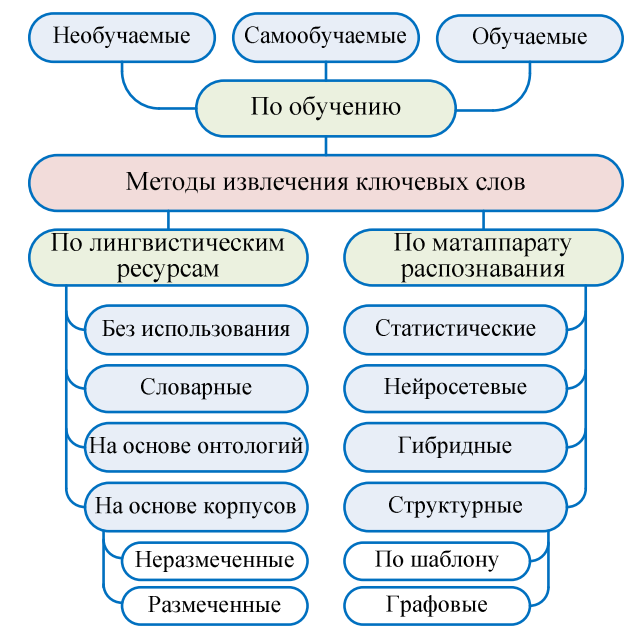
\includegraphics[width=0.7\linewidth]{src/img/ke_types}
	\caption[]{Классификация методов извлечения ключевых слов}
	\label{fig:ketypes}
\end{figure}

По второму признаку классификации прежде всего стоит выделить статистические и структурные методы извлечения КС.
Статистические методы учитывают относительные частоты встречаемости морфологических, лексических, синтаксических единици и их комбинации.
Это делает создаваемые на их основе алгоритмы довольно простыми, но недостаточно точными так как признак частотности ключевых слов не является превалирующим.
Одним из классических методов в данном классе является расчет для каждого слова меры, отражающей его важность в тексте, расматриваемого как элемент коллекции документов.

В основе структурных методов лежит представление о тексте как о системе семантически и грамматически взаимосвязанных элементов слов которые в свою очередь характеризуются набором лингвистических признаков.
По этому многие исследователи называют этот класс методов лингвистическим.
Здесь в первом приближении могут быть выделены два подкласса: графовые и синтаксически шаблонные методы.

Графовые или граф-ориентированные методы представляют текс множеством слов вершин или вершин словосочетаний и ребер отношений между ними.
Эти отношения могут выражать для каждой пары слов факты: последовательного появления в тексте, наличия в окне заданного размера и семантическую близость.
Для вершин полученного графа вычисляются меры центральности и по пороговому критерию отбираются ключевые слова.
Различия между данными методами состоят в особеностях учета значимости каждой вершины и вычисления отношений между ними.
В основе синтаксических шаблонных методов лежит представление о регулярных синтаксических конструкциях, содержащих на определенных позициях ключевые слова.
В чистом виде такие методы слабо применимы к расматриваемой задаче, могут использоваться в сочетании с другими.

Нейросетевые методы к задаче извлечения КС стали применяться стали применяться сравнительно недавно о основаны на свойстве искуственных нейронных сетей к обобщению и выделению скрытых зависимостей между входными и выходными данными.
Однако для формирования наборов данных для обучения и функционирования нейроных сетей требуется выделение структурных и статистических признаков, по этому на практике методы выделения КС являются гибридными т.е. сочетающими в себе элементы основных расмотренных класов.

Наконец алгоритмы извлечения КС, реализиющие означенные методы могут не использовать какие либо лигвистические ресурсы или исплользовать своего рода словари, онтологии, тезаурусы, а так же корпуса текстов с разметкой \cite{20}.

В данной работе не будут расматриваться методы требующие обучения или наличия корпуска текстов для обучения.

\subsection{TF-IDF}
TF-IDF представляет классическую числовую метрику которая показывает релевантность ключевого слова в рамках выбранного документа.
$TF$ (Term Frequency) частота термина равняются количеству повторений кандидата на общее количество слов в документе \eqref{eq:tf}.
$IDF$ (Inevrsed Document Frequency) инвертированная частота документа , используется для балансировки излишне повторяющихся слов \eqref{eq:idf}.
Представляет из натуральный логарифм от общее количетсво документов деленое на количество документов в которых найден термин-кандидат.
\begin{equation}
	\label{eq:tf}
	TF = \frac{N_t}{N_{all}}
\end{equation}
где $N_t$ - количество термина в документе; $N_{all}$ - колчество всех слов в документе

\begin{equation}
	\label{eq:idf}
	IDF = \log(N_d / D)
\end{equation}
где $N_d$ - количество документов в которых было найден кандидат; D - общее количество документов.

\subsection{Rake}
Rapid Authomatic Keyword Extraction (Rake) - это графовый метод использующий лингвистический подход "совместного появления" (сo-occurence) для извлечения ключевых слов из едининичного документа.
Не требует обучение, не зависит от предметеой области и языка документа.

Rake базируется на том что ключевые слова чаще всего представляют собой несколько слов и редко содержат пунктуацию и стоп слова такие как предлоги, речевые обороты и другие не значимые слова с минимальным лексическим значением. \cite{15}

\subsection{Yake}

Алгоритм Yake относится категории комбинированных методов, который испольует подходы как статистических методов так и графовых. 
Состоит из 4 главных шагов:

\begin{enumerate}
	\item предварительная обработка текста и определение термина-кандидата;
	\item извлечение свойств;
	\item вычисление счета термина;
	\item вычисление дублей и ранжирование.
\end{enumerate}
На первом шагу обрабатывается документ в машино-читаемый формат для определения потенциальных терминов-кандидатов.
Это важный и ключевой шаг от которого зависит качество определения кандидатов что на прямую влияет на эффективность самого алгоритма.
Следующей этап принимает на вход массив индивидуальных терминов и репрезентует их в виде набора статистических свойст.
На третьем этапе эти свойства эвристически объединяются в единую оценку которая отражает важность значения термина.
На финальном этапе сравниваются вероятно похожие термины на основе измерений схожести полученных от специальных алгоритмов.

Алгоритм на вход получает текст и необходимые параметры: размера окна w (используется для вычисления одного из статистических свойств), порог повторения $\theta$ и язык текста, последний строчный параметр используется для получения списка стоп слов.
Полученный текст метод начинает разделять на предложения.
Каждое предложение в результате предобработки превращается в некоторое количество терминов, что завершает первый этап.
На следущем шаге для каждого термина высчитываются его статистические свойства и подсчитывается оценка.
На завершаеющем шаге происходит отсеивание кандидатов на ключевое слово где свойсво схожести больше $\theta$.
Дальше список ключевых слов и оценки сортируются по релевантности и возвращаются данным методом, что завершает работу алгоритма.
Ниже приведено более детальное описание каждого шага.

\subsubsection{Предварительная обработка текста и определение списка кандидатов}
Предварительная обработка текста это первый этап после которого идет репрезентация текста и идет анализ текста.
На данном этапе идет очищение текста и трансформация его в машино-читаемый формат: выделены важные части и удалены шумовые слова.
Классическая предобработка включает в себя: очистку текста, разбиение на предложения, аннотирование текста, токенизацию и определение стоп слов.
Так же могут использоваться техники обработки текстов на естесетвенном языке (natural language processing, NLP): 
\begin{enumerate}
	\item пометка частей речи (part-of-speech tagging, PoS);
	\item распознавание именованных объектов (named-entity recognition, NER);
	\item нормализация;
	\item лингвистический разбор или стемминг;
\end{enumerate}
однако, для этого требуются специальные инструменты каждый работающий с языком для котого он был реализован.
В рамках этапа даного алгоритма они не используются.

\todo[inline]{Возможносто стоит заменить на выражение на русском языке}
Поступивший текст, алгоритм начинает делить на предложения. 
Это достигается путем применения сегментера текстов основанного на правилах, который разделяет индоевропейские языки на высказывания следую предопределенному шаблону.
На пример: "Python is awesome! But C++ is also very good" будет разделено на 2 выражения ("Python is awesome!", "But is awesome") в то время как "Mr. Smith" будет одиночным выражением.
Затем каждое высказывание делится на чанки (по найденой пунктуации) и затем проходит процесс токенизации.
Это очень важный этап который не только позволяет выделить слова, но и отсеить шум в виде пунктуации, электронных почт, и ссылок, который мешает при работе с огромными текстами.
После этого каждый токен приводится к нижнему регистру и помечаеся специльной меткой разделителем.

Результат предобработки это список выражений, разделенных на чанки, сформированных из помеченных терминов.
В следующем разделе приводится описание статистических свойств использующихся в данном методе.

\subsubsection{Вычисление свойсв}

После предварительной обработки и получения кандидатов применяется статистический анализ, который уделяет внимание структуре, частоте терминов и сочитаемости.
В начале создается пустая структура, которая будет хранить в себе одиночные термины, найденные в тексте и дополнительную информацию такую как результаты статистических метрик и оценку (вычисляется позже).
Затем перебираем список выражений и чанки.
Кажый чанк разбивается на ранее размеченные токены и для них вычисляются:
\begin{enumerate}
	\item частота термина (TF, term frequency);
	\item индес выражений, где встречается данный токен (offsets\_sentences);
	\item частота акронима термина (TF\_a, term frequency of acronym);
	\item частота слова в старшем регистре (TF\_U, term frequency of uppercase);
\end{enumerate}
в дополнении к ним так же вычисляются матрица сочитаемости для сохранения связи между термином и его предшествеником или подтермины найдены в окнем размером w.
После того, как статистика каждого термина вычислена, теперь можно проводить процесс извлечения признаков.
Дли одиночного термина извлекаются следующие признаки: TCase, TPos, TFNorm, Trel и Tsent, детальное описание каждого признака идет ниже.

\subsubsection{Регистр ($T_{Case}$)}

Аспект термина связанный с регистром является важной характеристикой при рассмотрении извлечения ключевых слов.
Основаня идея что термины в верхнем регистре, как правило, более релевантны, чем слова в нижнем регистре. 
В представленом подходе мы уделяем особое внимание любому термину, начинающийся с заглавной буквы (исключая начало предложений), темболее аббревиатуры где все буквы слова заглавные.
Однако вместо того, чтобы считать это двойным весом, мы будем рассматривать только максимальное вхождение в пределах двух из них. 
Уравнение \eqref{eq:tcase} отражает внешний вид термина-кандидата:
\begin{equation}
	\label{eq:tcase}
	T_{Case} = \frac{max(TF(U(t))), TF(A(t))}{ln(TF(t))}
\end{equation}
где $TF(U(t))$ количетсво термина-кандидата t нающегося с залавной буквы, $TF(A(t))$ сколько раз кандидат t был отмечен как акроним и $TF(t)$ - это частота t.
Таким образом чем чаще кандидат пишется с заглавной буквы, тем более важным он считаетсся.
Это означает, что термин-кандидат, встречающийся с заглавной буквой 10 из 10 случаев будет иметь большее значение чем коллега встретившийся 5 раз из 5 случаев.

\subsubsection{Позиция термина ($T_{position}$)}
Другим индикатором важности кандидата является позиция.
Причина в том, что релевантные слова, как правило, появляются в самом начале документа, тогда как слова, встречающиеся в середине или в конце документа, имеют тенденцию быть менее важными.
Особенно это очивидно как для новостных статей, так и для научных текстов, двух видов публикаций, которые склонны концентрировать большое количество важных ключевых слов вверхней части текста.
На пример в ведении или в аннотации.
Предположение авторов состоит в том, что термины, встречающиеся в первых предложениях текста должны быть более высоко оценены, чем термины, которые появляются позже. 
Таким образом, вместо того, чтобы рассматривать равномерное распределение терминов,
их модель присваивает более высокие баллы терминам, встречающимся в первых предложениях. 
Вес рассчитывается, используя следующее уравнение \eqref{eq:tposition}:
\begin{equation}
	\label{eq:tposition}
	T_{position} = ln(ln(3 + Median(Sen_t)))
\end{equation}
где $Sen_t$ множество позий в выражениях где кандидат t появляется и медиана от $Sen_t$.
Зная что медианая функция $Median(Sen_t)$ может возвращать значение 0 (когда термн-кандидат появляется только в первом предложении), к уравнению добавляются константа $C > e$, в случаи данной реализации 3 (как первое число после $e$), что бы гарантировать что $T_{position} > 0$.
Так же для сглаживания разницы между терминами, с большой средней разницы используется двойной логарифм.

Так для термина-кандидата $t_1$ который появляется в 2, 35, 70, 74, 4000 выражениях в документе будет иметь $T_{position} = ln(ln(3 + Median(2, 35, 70, 74, 4000))) = 1.45$ в то время как $t_2$, появляющийся в 1, 4 и 7 выражении получит $T_position = ln(ln(3 + Median(1, 4, 7)) = 0.66$.
Результатом является возрастающая функция, значения которой имеют тенденцию плавно возрастать по мере того, как термин-кандидаты располагаются ближе к концу документа, а это значит, что чем больше кандидатов появляются в начале документа, тем ниже его значение $T_{position}$ и наоборот терминам (менее актуальные), расположеным ближе к концу документа будет присвоено более высокое значение $T_position$.

\subsubsection{Нормализация частоты термина ($TF_{norm}$)}
Это функция указывает частоту  термина-кандидата $t$ в документе на основе работе Луна \cite{18}, которая утверждает что "частота появления слова в тексте обеспечивает полезное измерение значения слова".
Данное высказывание отобржает убеждение, что чем выше частота кандидата, тем выше его важность.
Тем не менее, это не означает что важность пропорциональна тому сколько раз встречается термин.
Таким образом для предотвращения смещения в сторону высоких частот в длинных документах значение $TF$ кандидата $t$ делится на среднее значение частот (MeanTF) плюс 1, умноженное на старднтное отклонение \eqref{eq:tfnorm}.

\begin{equation}
	\label{eq:tfnorm}
	TF_{norm} = \frac{TF(t)}{MeanTF + 1 * \sigma}
\end{equation} 
Цель заключается в том, что бы оценить все термины-кандидаты, частоты которых выше среднего, сбалансированого определенной степенью дисперсии, заданная стандартным отклонением.
Что бы вычислить это авторы метода решили учитывать только MeanTF и стандартое отклонение не стоп-слов, что гарантирует, что на вычисления этих двух компонентов не влияют высокие частоты, регистрируемые по стоп-словам.

\subsubsection{Связь термина с контекстом}
Хотя стоп-слова представляют собой бесспорно полезный источник знаний о том, что явно не относится к делу, только полагаясь на статическом списке,информации может оказаться недостаточно для отбрасывания нерелевантных слов.
В данном разделе описываюется статистическая функция, которая нацелена на определение дисперсии (D) термина-кандидата t относительно его конкретного контекста, опирающаяся на работу Machado \cite{19}, утвержающая что чем выше число различных терминов, которые встречаются вместе с термин-кандидатом t c обеих сторон, тем менее значимым быдет термин t

\begin{figure}[!h]
	\centering
	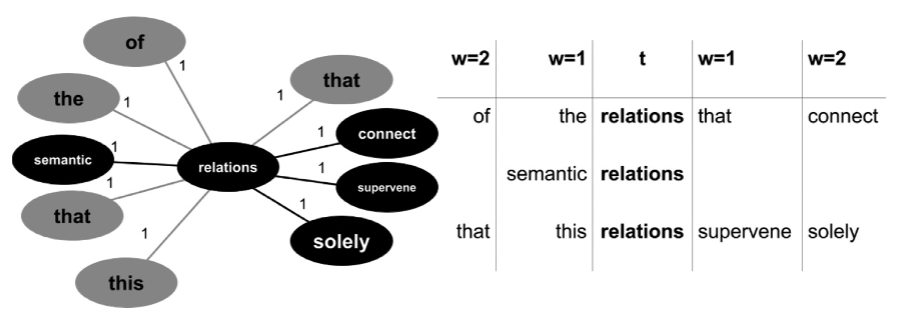
\includegraphics[width=1\linewidth]{src/img/coocurrences_example}
	\caption{Совместное появление при w = 2}
	\label{fig:coocurrencesexample}
\end{figure}

\begin{equation}
	DL[DR] = \frac{|A_t, w|}{\sum_{k \in A_{t, w}CoOccur_{t, k}}} 
\end{equation}
где $|A_t, w|$ представляет собой количество различных терминов, где термин представляет собой анализируемое содержимое, аббревиатуру, или слово в верхнем регистре, которое появляется слева(справа) от термина-кандидата t в заданном окне размера w \eqref{fig:coocurrencesexample} в отношении k терминов с которыми он встречается.

Затем DL и DR умножаются на частоту термина-кандидата, деленную на максимальную частоту термина среди всех кандидатов, которые встречаются в документе.
Окончательное уравнение имеет вид \eqref{eq:trel}:
\begin{equation}
	\label{eq:trel}
	T_{Rel} = 1 + (DL + DR) * \frac{TF_t}{MaxTF}
\end{equation}
где крайняя левая часть уравнения измеряет значимость термина-кандидата по отношению к его левой части, а
самая правая часть измеряет свою значимость по отношению к правой стороне. С практической точки зрения, чем менее релевантен кандидат t, тем выше будет оценка этой функции.
Таким образом, стоп-слова и, аналогичным образом, недискриминационные термины, как правило, получают более высокий балл. На рис. \eqref{fig:coocurrencesexample} показаны различные термины, которые встречаются вместе с термином-кандидатом «relations» в пределах w, равного 2, где «relations» — неважный термин (не часть истины, т. е. не золотое ключевое слово) в контексте нашего текущего примера.
В правой части рисунка показаны отрывки из текста, в которых встречается термин «отношения», а в левой — графическое представление. 
Число на ребрах — это частота, с которой термин-кандидат «relations» встречается вместе в соответствующем овале. 
Серым цветом обозначены стоп-слова.

\subsubsection{Другое предложение термина ($T_{sentence}$)}

Это свойство подсчитывает как часто термин-кандидат встречает в других предложениях.
Оно отображает, что кандидат, встречающийся во многих других предложениях, можеть быть более важным.
Оценка подчитывается по следующей формуле:

\begin{equation}
	T_{sentence} = \frac{SF(t)}{Sentences}
\end{equation}
где $SF(t)$ - количество предложений в которых появляется t.
$Sentences$ - это максимальное количесвто предолжений в тексте.
Результат лежит в диапозоне от $[0, 1]$


\subsubsection{Подсчет оценки термина}
После того как все оценки свойст получены, можно подсчитать финальный результат оценки термина.
Все полученные ранее оценки подставляются в выражение S(t) \eqref{eq:termin_score}.

\begin{equation}
	\label{eq:termin_score}
	S(t) = \frac{T_{Rel} * T_{Postion}}{T_{Case} + \frac{TF_{Norm}}{T_{Rel}} + \frac{T_{sentences}}{T_{Rel}}}
\end{equation}
Стоит обратить внимание на то что $TF_{Norm}$ и $TF_{sentensec}$ делятся на $T_{Rel}$.
Это делается для того что бы присвоить большое значение терминам, которые появляются часто во многих предложениях, до тех пор пока они релевантны.
По скольку, некоторые кандидаты могут встрчаться много раз в многих предложениях и при этом быть бесполезными и должны быть оштрафованы.
Таким образом достижение высокой оценки по $TF_{Norm}$ и $TF_{sentensec}$ является индикацией важности термина при низком значении $T_{Rel}$.
Так же важным свойством является является свойство позиции появления термина, она добавляется в выражение путем умножения $T_{Rel} * T_{Postion}$

\subsection{Сравнение методов}
\begin{enumerate}
	\item TF-IDF
	\item Плюсы \begin{enumerate}
		\item простой.
	\end{enumerate}
	\item Минусы \begin{enumerate}
		\item требует наличия большого корпуса текстов;
		\item не работает с словосочитаниями
		\item оценка происходит только по частотной характеристеке термина
	\end{enumerate}
	\item Rake
	\item Плюсы \begin{enumerate}
		\item простой
		\item не требует корпус текстов;
		\item учитывает взаимосвязи слов в тексте.
	\end{enumerate}
	\item Минусы \begin{enumerate}
		\item оценка происходит только по частотной характеристеке термина
		\item не выдает словосочитания
	\end{enumerate}
	\item Yake
	\item Плюсы \begin{enumerate}
		\item учитывает взаимосвязи слов;
		\item учитывает позицию кандидата;
		\item учитывает его написание (абревиатуры, регистры);
		\item учитывается связь с контекстом
	\end{enumerate}
	\item Минусы \begin{enumerate}
		\item Не выдает словосочитания
	\end{enumerate}
\end{enumerate}

Учитывая все ранее выставленные требования к алгоритмам и выведенные их сильные и слабые стороны было принято решение использовать метод Yake.
До этого данный метод не спользовался для вычисления ключевых слов из текста на русском языке и для этого необходимо провести следующие модификации:
\begin{enumerate}
	\item добавление сборника стоп-слов;
	\item добавление работы с N-gram;
\end{enumerate}

\subsection{Модификация}
Шумовые слова (или стоп-слова) — термин из теории поиска информации по ключевым словам.
Это такие слова, знаки, символы, которые самостоятельно не несут никакой смысловой нагрузки, но
которые, тем не менее, совершенно необходимы для нормального восприятия текста, его целостности.
К ним относятся предлоги, суффиксы, причастия, междометия, цифры, частицы и т. п.
Так как данные слова имеют самые большие частоты встречи в документах, то для более корректного результата небходимо данные слова исключать из текста, по этому есть необходимость в добавлении в метод списка стоп-слов для русского языка.

Как было описано ранее, результатом работы метода Yake являются одиночные ключевые слова с оценкой.
Современные технологии непрерывано развивиются.
Это значительно влияет на научно-технический функциональный стиль, в частности, на его терминосистемы.
Появляются новые термины и усложняются старые \cite{22}.
В результате растет количество многокомпонентных терминов.
По этому есть необходимость в модификации выбранного метода для возможность извлечения мнокомпонентных ключевых слов.
Данную модификацию проведем с помощью добавления n-грамм.
Пусть задан некоторый конечный алфавит $V = {w_i}$, где $w_i$ - символ. 
Языком $L(V)$ называют множество цепочек конечной длины из символов $w_i$.
Высказыванием называют цепочку из языка.
N-граммой на алфавите V называют произвольную цепочку длинной N, например последовательность из N букв русского языка, одного слова, одной фразы, одного текста \cite{21}.

Конечный результат будет высчитываться по формуле \eqref{eq:ngram}: 
\begin{equation}
	\label{eq:ngram}
	S(kw) = \frac{\prod_{t \in kw}S(t)}{KF(kw) * (1 + \sum_{t \in kw}S(t))}
\end{equation}
где $S(kw)$ - финальный результат оценки, чем ниже тем реливантнее, $S(t)$ - оценка одиночного термина,
$KF(kw)$ - частота ключевого слова(выражения)

\subsection{Заключение}
В рамках данного раздела представлено описание предметной области задачи по извлечению ключевых слов. Приведена систематизация методов извлечения КС и текстов.
Произведен отбор и сравнение методов удовлетворяющих выставленным ограничениям.
Представлена модификация метода Yake


